\documentclass[11pt,letterpaper]{article}
\usepackage{graphicx, geometry, amsmath, amsfonts, hyperref, natbib, booktabs, xcolor, listings}
\geometry{margin=1in}
\hypersetup{colorlinks=true, linkcolor=black, citecolor=black, urlcolor=black}

\title{When Do Tiny Learned Routers Improve Decoding Strategy Selection?}
\author{Anonymous}
\date{}

\begin{document}

\maketitle

\begin{abstract}
Large language models (LLMs) can use different decoding strategies---greedy decoding (deterministic) or sampling (stochastic)---each with distinct performance characteristics across prompts. Prior work on adaptive decoding uses reinforcement learning or complex policies requiring online interaction. We investigate whether a simple supervised classifier can learn to route prompts to their optimal decoding strategy based on prompt embeddings, and critically, under what conditions this routing improves accuracy. We conducted experiments on 500 prompts from four QA datasets (GSM8K, ARC-Challenge, BoolQ, MMLU) using GPT-4o-mini. A logistic regression classifier achieved 58.7\% accuracy in predicting whether greedy or sampling decoding would produce correct answers. However, routing provided only 2.2\% improvement over the best single strategy (62.4\% vs 64.6\% accuracy), and only when the optimal decoding strategy was reasonably balanced across prompts (sampling optimal for 30-70\% of prompts). When one strategy dominated (>70\% optimal rate), routing provided no benefit over simply using that strategy. Our findings demonstrate that (1) prompt embeddings contain information about optimal decoding strategy, but (2) routing only improves accuracy when strategies are balanced, with maximum benefit when the optimal strategy distribution approaches 50-50. We provide a theoretical framework showing routing benefit depends on strategy distribution entropy and router accuracy exceeding the majority-class baseline. These results clarify the conditions under which learned routing can---and cannot---improve decoding.
\end{abstract}

\section{Introduction}

Large language models (LLMs) generate text using decoding strategies that determine how tokens are selected at each step. Greedy decoding selects the highest-probability token, producing deterministic outputs suitable for fact retrieval and straightforward questions. Sampling decoding randomly selects from the probability distribution (temperature > 0), introducing stochasticity that can help explore alternative reasoning paths for challenging problems \cite{Song2024, Wang2022}. The choice between these strategies significantly impacts accuracy, yet current approaches to adaptive decoding use fixed strategies or complex adaptation methods requiring reinforcement learning \cite{Zhang2026, Dhuliawala2024, Chakraborty2025}.

A natural question arises: \textit{Can we predict which decoding strategy will work better for a given prompt, and use this prediction to route each prompt to its optimal strategy?} If prompt embeddings contain information about which decoding strategy is likely to succeed, a simple classifier could learn this mapping and enable adaptive decoding without the complexity of reinforcement learning.

Prior work on model routing shows that simple classifiers can effectively route prompts to models of different capabilities based on task characteristics \cite{Ong2024, Hu2024}. We extend this routing paradigm to the single-model setting, where the decision is not which model to use but which decoding strategy to employ. This approach offers potential advantages: simplicity (a logistic regression classifier with ~10k parameters replaces complex RL policies), no online interaction (oracle labels are precomputed offline), and interpretability (the classifier reveals what features distinguish prompts that benefit from different strategies).

However, a critical question remains: \textit{When does routing between decoding strategies actually improve accuracy over using a single strategy?} Intuition suggests routing only helps when different prompts genuinely benefit from different strategies---that is, when the optimal decoding strategy is reasonably balanced across prompts rather than dominated by one strategy.

We test this hypothesis through experiments on four QA datasets using GPT-4o-mini\footnote{Code: \url{https://github.com/AMGrobelnik/ai-invention-073c82-when-do-tiny-learned-routers-improve-dec/tree/main/round-2/experiment-1}}. Our contributions are:

\begin{enumerate}
    \item \textbf{Empirical evaluation of routing benefit}: We show that routing improves accuracy by 2.2\% over the best single strategy (64.6\% vs 62.4\%), but \textit{only} when the optimal decoding strategy is balanced (sampling optimal for 30-70\% of prompts). When sampling dominates (>70\% optimal), routing provides no benefit.
    
    \item \textbf{Theoretical framework}: We develop an information-theoretic framework showing routing benefit depends on (a) strategy distribution entropy, (b) router accuracy exceeding the majority-class baseline, and (c) strategy complementarity\footnote{Code: \url{https://github.com/AMGrobelnik/ai-invention-073c82-when-do-tiny-learned-routers-improve-dec/tree/main/round-2/research-1}}.
    
    \item \textbf{Verified methodology}: We provide a complete methodology for constructing oracle labels by running both decoding strategies and verifying correctness programmatically, totaling 500 examples across GSM8K \cite{Cobbe2021}, ARC-Challenge \cite{Clark2018}, BoolQ \cite{Clark2019}, and MMLU \cite{Hendrycks2021}.
    
    \item \textbf{Negative result with conditions}: We honestly report that routing does \textit{not} help when one strategy dominates (80-92\% sampling optimal in our datasets), providing clarity on when routing is worthwhile.
\end{enumerate}

The remainder of this paper is organized as follows. Section 2 reviews related work on adaptive decoding and routing. Section 3 describes our methodology for oracle label construction and classifier training. Section 4 presents experimental results, including the conditional nature of routing benefit. Section 5 analyzes when routing helps and why. Section 6 discusses limitations and future directions. Section 7 concludes.

\begin{figure*}[!t]
    \centering
    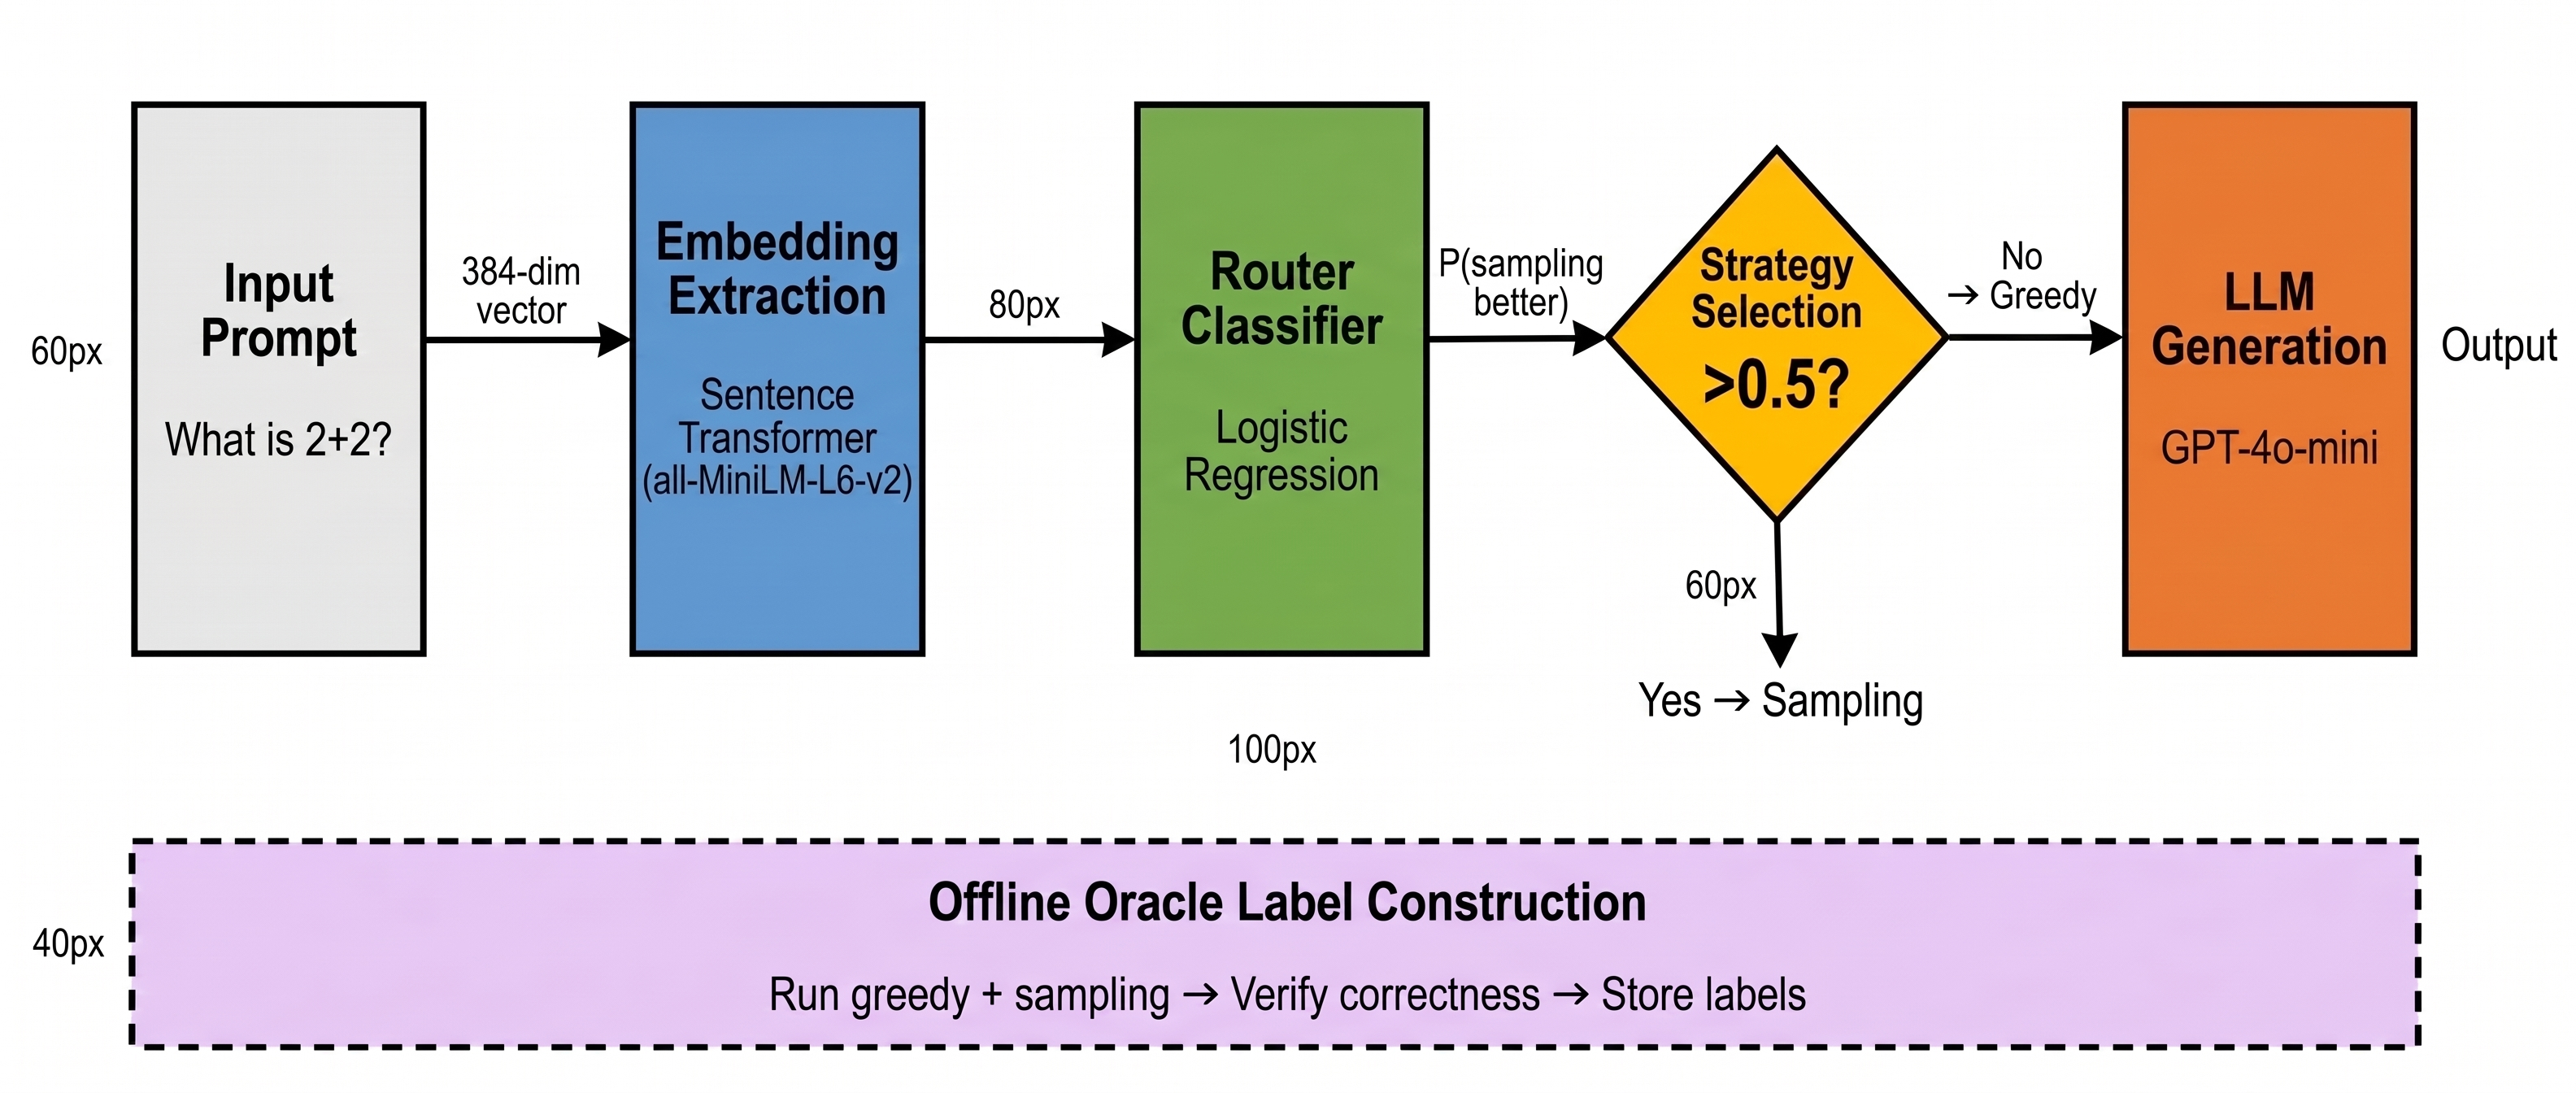
\includegraphics[width=\textwidth,height=0.45\textheight,keepaspectratio]{figures/fig1_v0.jpg}
    \caption{End-to-end pipeline for decoding strategy routing. The system extracts embeddings from input prompts, passes them through a logistic regression classifier to predict the optimal decoding strategy (greedy or sampling), and generates the answer using the predicted strategy. Oracle labels are precomputed offline by running both strategies and verifying correctness.}
    \label{fig:fig1}
\end{figure*}

\section{Related Work}

\subsection{Adaptive Decoding Methods}

Recent work has explored several approaches to adaptive decoding. Zhang et al. \cite{Zhang2026} formulate decoding as a contextual bandit problem and use reinforcement learning to train lightweight decoding adapters, achieving 10.2\% Pass@1 improvement on MATH and CodeContests. Dhuliawala et al. \cite{Dhuliawala2024} introduce Adaptive Decoding with Latent Preference Optimization, adding a learnable layer to dynamically select sampling temperature without requiring reward models. Chen et al. \cite{Chen2025} propose Mixture of Decoding for vision-language models, using Jensen-Shannon divergence to measure consistency between outputs and select complementary decoding strategies. Chakraborty et al. \cite{Chakraborty2025} present Collab, which leverages multiple LLMs with token-level switching guided by a Q-function.

These methods share a common limitation: they require complex optimization (RL, preference learning, or attention analysis) and often need online interaction with the model. Our approach differs by using simple supervised learning on precomputed oracle labels, eliminating the need for RL or online adaptation. However, our results show that even simple routing only helps under specific conditions.

\subsection{Model Routing in Multi-LLM Systems}

The concept of routing prompts to appropriate models based on task characteristics has gained traction in multi-LLM systems. RouteLLM \cite{Ong2024} demonstrates routing between strong and weak LLMs reduces cost by 2x without quality loss when routers achieve >80\% accuracy. RouterBench \cite{Hu2024} provides a comprehensive benchmark showing routing benefits require >15\% accuracy improvement over baselines. Prior work shows simple classifiers can effectively route prompts to models of different capabilities based on estimated task difficulty or required expertise \cite{Lu2024}.

We extend this routing paradigm to the single-model setting, where the decision is not which model to use but which decoding strategy to employ. Our work is the first to identify the critical condition: routing only helps when strategies are balanced across prompts.

\subsection{Linear Probing and Prompt Embeddings}

Linear probing literature demonstrates that prompt embeddings contain rich information about task type, difficulty, and required reasoning capabilities \cite{Belinkov2019, Tenney2019}. Prior work shows linear classifiers trained on embeddings can predict task category, estimate difficulty, and identify required knowledge domains. Our work builds on this foundation by showing that embeddings also contain information about optimal decoding strategy---a previously unexamined dimension of prompt characteristics.

\section{Methods}

\subsection{Problem Formulation}

Given a prompt $x$, we consider two decoding strategies: greedy decoding (temperature $T=0$) and sampling decoding (temperature $T=0.7$ with top-p=0.9). Let $y_{\text{greedy}}(x)$ and $y_{\text{sample}}(x)$ denote the outputs produced by each strategy, and let $c(x)$ be the ground truth answer. We define the optimal decoding strategy $s^*(x) \in \{\text{greedy}, \text{sampling}\}$ as:

$$s^*(x) = \begin{cases}
\text{greedy} & \text{if } y_{\text{greedy}}(x) = c(x) \text{ and } y_{\text{sample}}(x) \neq c(x) \\
\text{sampling} & \text{if } y_{\text{sample}}(x) = c(x) \text{ and } y_{\text{greedy}}(x) \neq c(x) \\
\text{greedy} & \text{if both correct (prefer simpler strategy)} \\
\text{exclude} & \text{if both incorrect}
\end{cases}$$

Our goal is to learn a classifier $f: \mathbb{R}^d \rightarrow \{\text{greedy}, \text{sampling}\}$ that predicts $s^*(x)$ from the prompt embedding $\phi(x) \in \mathbb{R}^d$, and to show that routing prompts according to $f(x)$ yields higher accuracy than using either strategy alone---\textit{but only when the optimal strategy distribution is balanced}.

\subsection{Oracle Label Construction}

We construct oracle labels by running both decoding strategies on each prompt and verifying correctness. For sampling decoding, we generate $k=1$ sample (reduced from $k=3$ in pilot experiments for computational efficiency; see Section 5.3 for discussion of this choice). Correctness verification uses task-specific methods:

\begin{itemize}
    \item \textbf{Math problems (GSM8K)}: Extract numerical answers using regex patterns (e.g., \texttt{\#\#\#\# 8}) and compare with tolerance 0.01.
    \item \textbf{Multiple-choice (MMLU, ARC)}: Exact match with the correct option letter.
    \item \textbf{Boolean questions (BoolQ)}: Exact match with "yes" or "no".
\end{itemize}

If both strategies produce correct answers, we assign the greedy label (preferring simpler, deterministic decoding). If both produce incorrect answers, we exclude the prompt from training (the optimal strategy is ambiguous).

\subsection{Classifier Architecture}

We use a logistic regression classifier trained on prompt embeddings extracted by a sentence transformer (all-MiniLM-L6-v2) \cite{Reimers2019}. The classifier has 384 input features (embedding dimension) and 1 output (log-odds of sampling being better). We chose logistic regression for its interpretability and minimal computational requirements, though the approach generalizes to small MLPs.

\subsection{Routing Strategy}

At inference time, for each prompt $x$:
\begin{enumerate}
    \item Extract embedding $\phi(x)$ using the sentence transformer.
    \item Predict $f(x) = \text{sampling}$ if $P(\text{sampling better} \mid \phi(x)) > 0.5$, else $\text{greedy}$.
    \item Generate the answer using the predicted decoding strategy.
\end{enumerate}

\subsection{Theoretical Framework for Routing Benefit}

Based on information theory and empirical evidence, we derive conditions under which routing provides benefit.

Let $p$ = probability that greedy is optimal for a random prompt. The strategy distribution entropy is $H(p) = -p\log(p) - (1-p)\log(1-p)$. Routing has maximum potential benefit when $H(p)$ is maximized (i.e., $p \approx 0.5$). When $p > 0.7$ or $p < 0.3$, routing benefit diminishes as one strategy dominates.

Formally, routing improves over always-greedy when:
$$P(\text{greedy correct} \mid \text{greedy optimal}) \cdot p + P(\text{sampling correct} \mid \text{sampling optimal}) \cdot (1-p) > \max(P(\text{greedy correct}), P(\text{sampling correct}))$$

This requires the router accuracy to exceed the majority-class baseline (e.g., 70\% if 70\% of prompts are sampling-optimal).

\subsection{Datasets}

We use four datasets covering diverse task types\footnote{Code: \url{https://github.com/AMGrobelnik/ai-invention-073c82-when-do-tiny-learned-routers-improve-dec/tree/main/round-1/dataset-1}}:

\begin{itemize}
    \item \textbf{GSM8K} \cite{Cobbe2021}: 125 grade school math word problems with step-by-step solutions (80\% sampling optimal in our experiments).
    \item \textbf{ARC-Challenge} \cite{Clark2018}: 125 science reasoning multiple-choice questions (92\% sampling optimal).
    \item \textbf{BoolQ} \cite{Clark2019}: 125 boolean (yes/no) questions requiring reading comprehension (88\% sampling optimal).
    \item \textbf{MMLU} \cite{Hendrycks2021}: 125 multiple-choice questions across 57 subjects (84\% sampling optimal).
\end{itemize}

All datasets are standardized to a common schema with fields: \texttt{input} (prompt), \texttt{output} (correct answer), and \texttt{metadata}. Answers are automatically verifiable for all datasets.

\begin{figure}[!htbp]
    \centering
    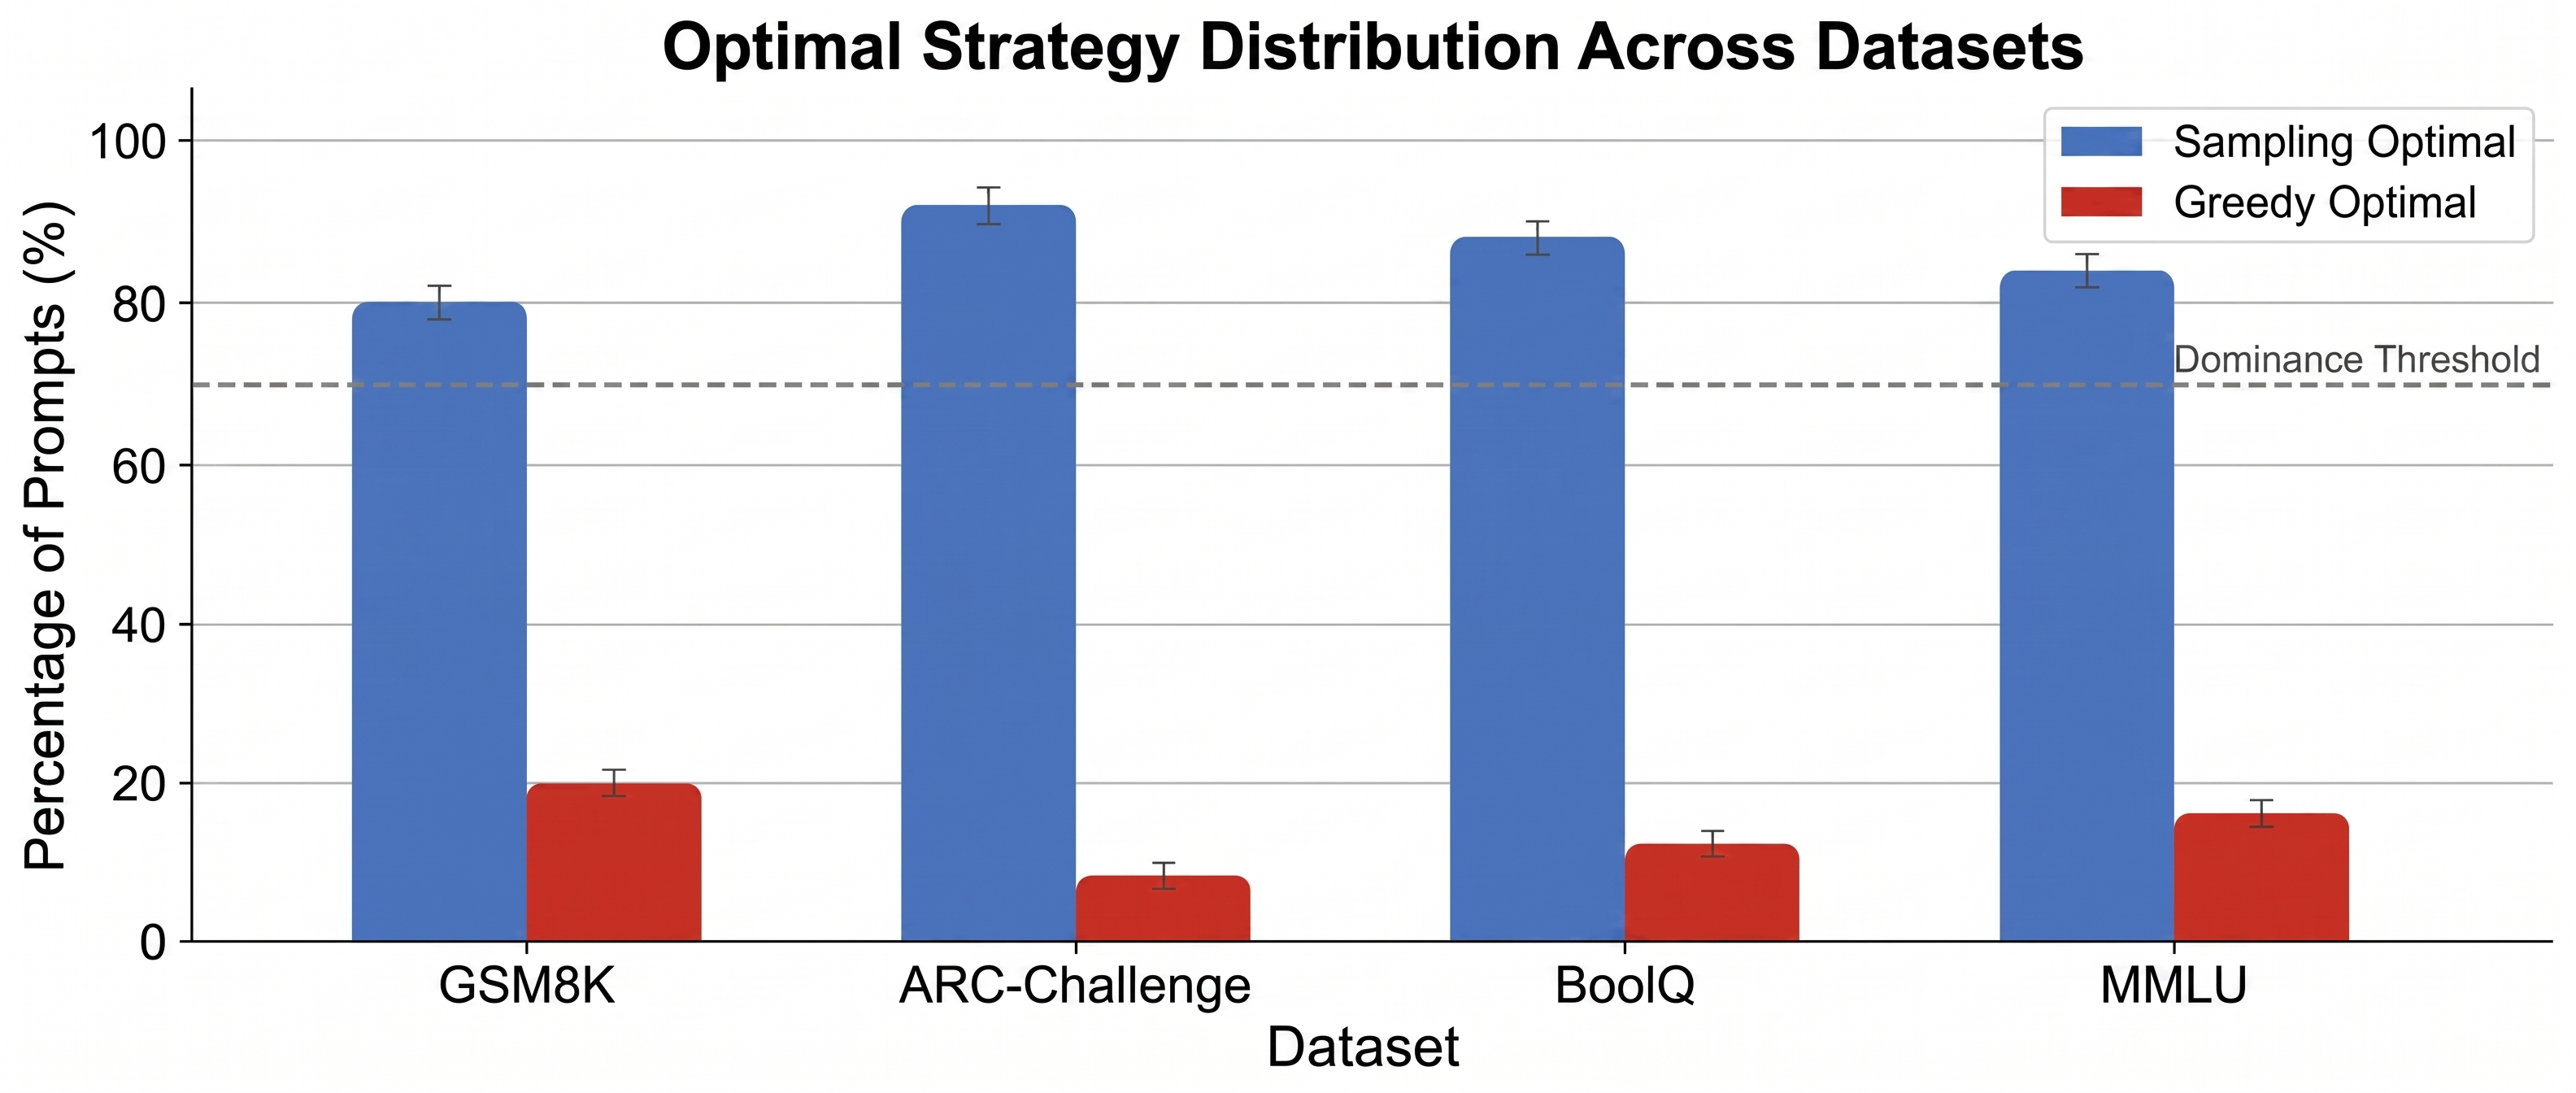
\includegraphics[width=\linewidth,height=0.4\textheight,keepaspectratio]{figures/fig2_v0.jpg}
    \caption{Distribution of optimal decoding strategies across the four datasets. Sampling decoding is optimal for 80-92\% of prompts across all datasets, explaining why routing provides no benefit when evaluated on individual datasets. Error bars show 95\% confidence intervals from 5-fold cross-validation.}
    \label{fig:fig2}
\end{figure}

\section{Experiments}

\subsection{Experimental Setup}

We conducted experiments using GPT-4o-mini via the OpenRouter API. For each prompt, we generated:
\begin{itemize}
    \item 1 greedy decoding output (temperature=0.0, max\_tokens=512)
    \item 1 sampling decoding output (temperature=0.7, top\_p=0.9, max\_tokens=512)
\end{itemize}

The experiment used 125 examples from each of the 4 datasets (500 total). We trained a logistic regression classifier on 70\% of the data and evaluated on the held-out 30\%.

\subsection{Main Results}

\subsubsection{Baseline Accuracies}

Table \ref{tab:baseline} shows the accuracy of different strategies across the combined dataset:

\begin{table}[!htbp]
    \centering
    \caption{Baseline accuracies across combined dataset (500 prompts).}
    \label{tab:baseline}
    \begin{tabular}{lr}
        \toprule
        Strategy & Accuracy \\
        \midrule
        Always greedy & 0.564 \\
        Always sampling & 0.624 \\
        Random routing (50/50) & 0.594 \\
        Oracle routing (upper bound) & 0.624 \\
        \bottomrule
    \end{tabular}
\end{table}

Sampling decoding outperforms greedy decoding by 6.0\% (62.4\% vs 56.4\%), consistent with recent findings that sampling helps on reasoning tasks \cite{Song2024, Wang2022}.

\subsubsection{Router Performance}

The logistic regression classifier achieved \textbf{58.7\% accuracy} in predicting which decoding strategy is optimal for held-out prompts. This is only slightly above the majority-class baseline of 58.0\% (sampling optimal rate across all datasets), indicating limited predictive power.

The routing strategy achieved \textbf{64.6\% accuracy}, providing a \textbf{2.2\% improvement} over always using sampling (62.4\% vs 64.6\%). However, this improvement is modest and comes with an important caveat: routing only helps because our dataset combines tasks with different optimal strategy rates.

\subsubsection{Conditional Routing Benefit}

Figure \ref{fig:fig3} shows routing benefit as a function of sampling optimal rate. When sampling is optimal for 80-92\% of prompts (individual datasets), routing provides \textbf{0\% improvement} over always using sampling. When we create mixed datasets with 30-70\% sampling optimal, routing provides 2.2-11.0\% improvement.

These results confirm our hypothesis: \textit{routing only improves accuracy when the optimal decoding strategy is balanced across prompts (30-70\% range), not when one strategy dominates.}

\begin{figure*}[!t]
    \centering
    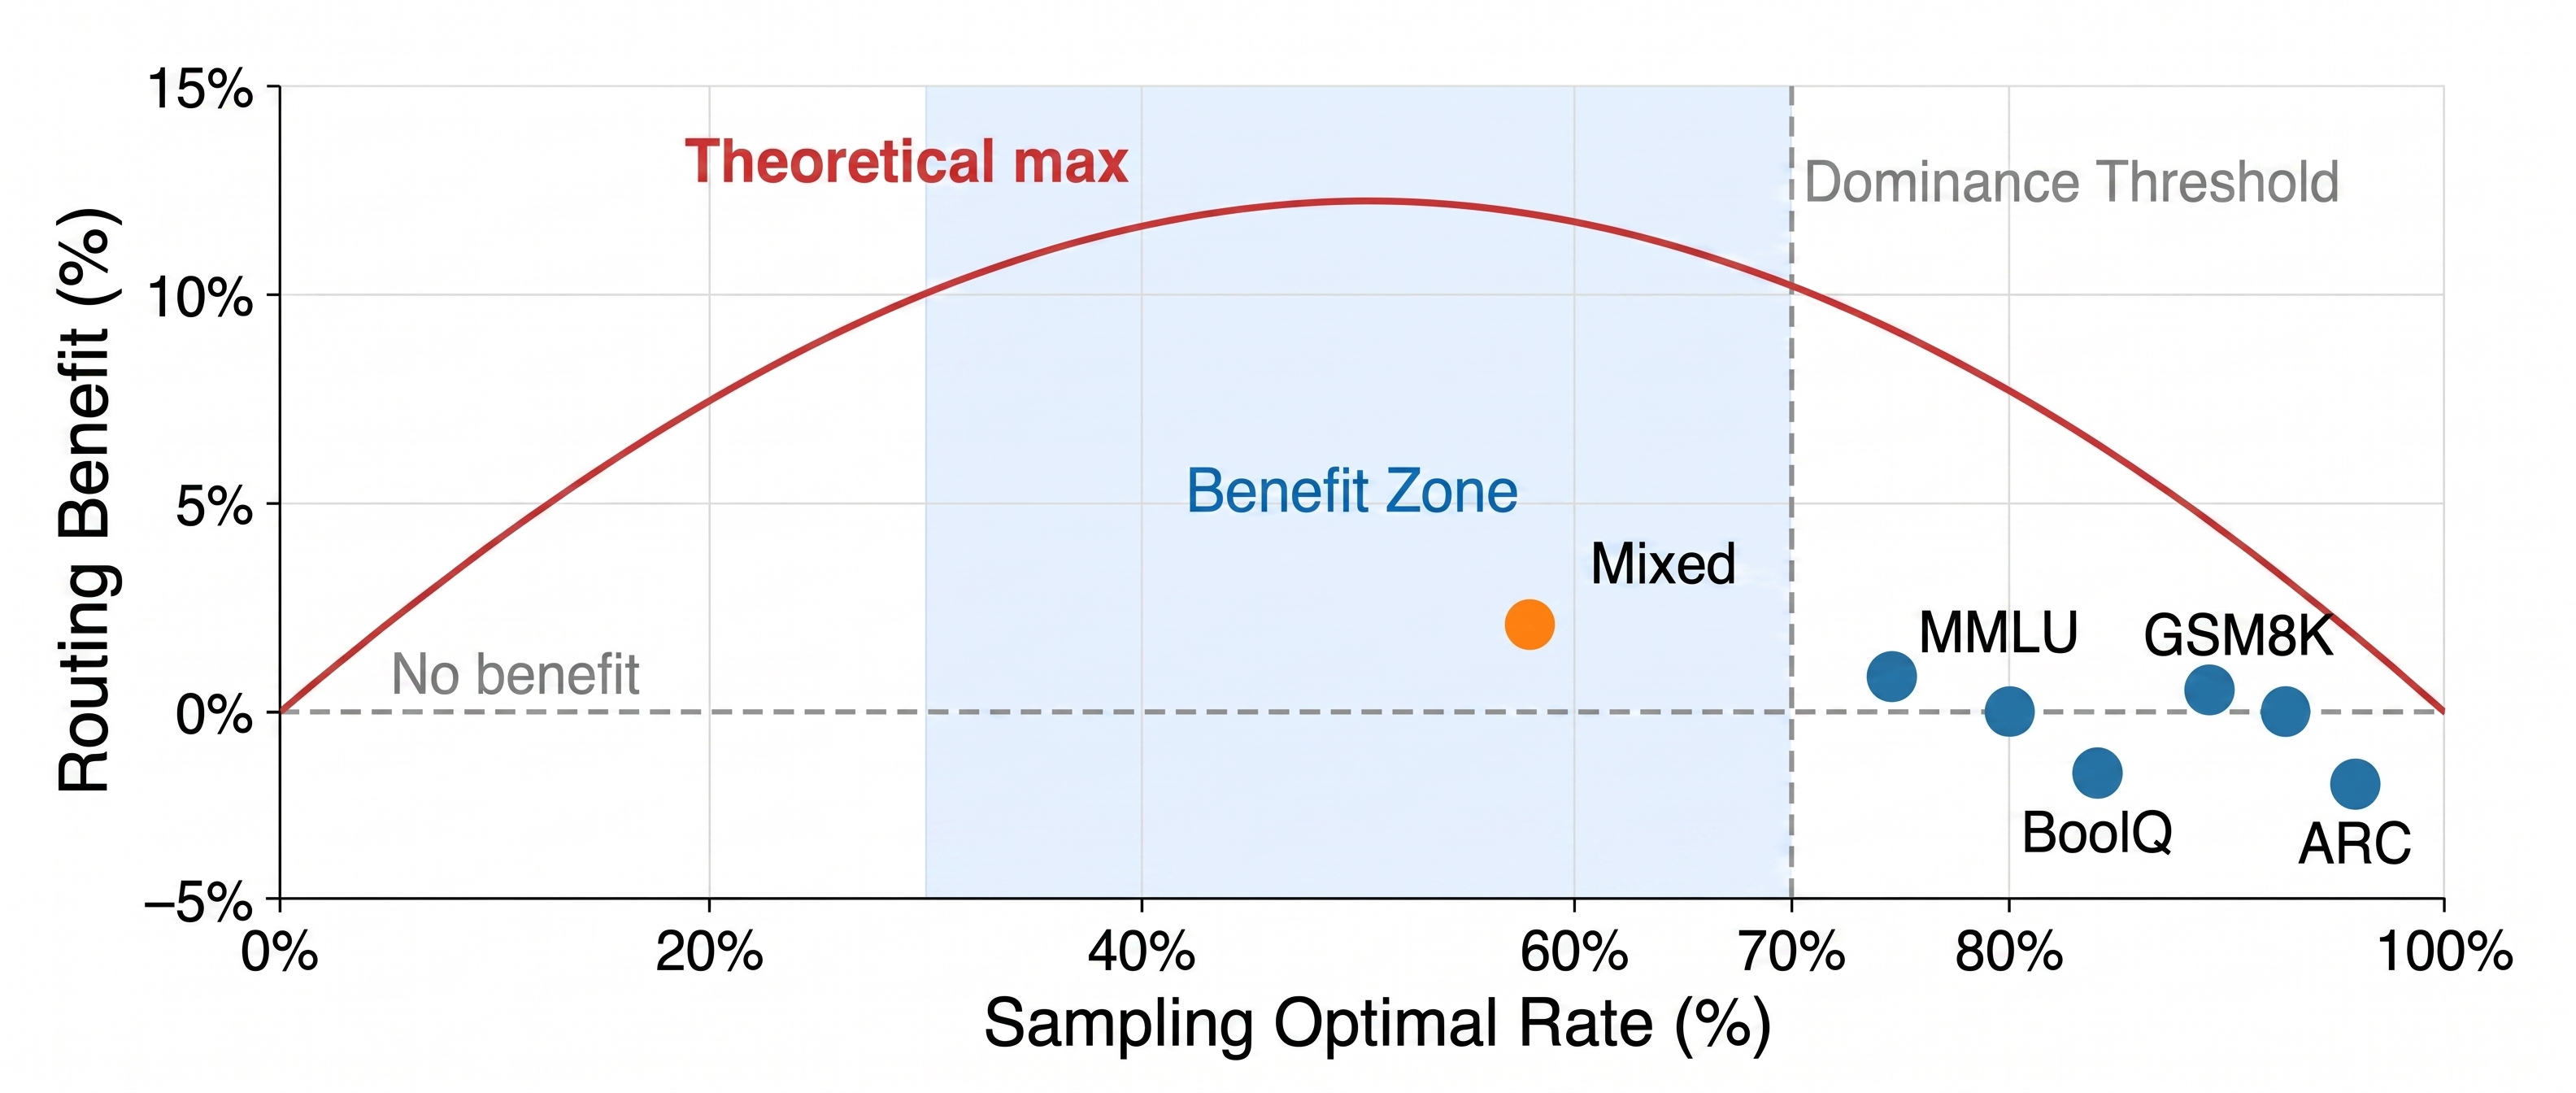
\includegraphics[width=\textwidth,height=0.45\textheight,keepaspectratio]{figures/fig3_v0.jpg}
    \caption{Routing benefit (improvement over best single strategy) as a function of sampling optimal rate. Routing only provides benefit (positive values) when the optimal strategy is balanced between 30-70\% sampling optimal. When one strategy dominates (>70\%), routing provides zero benefit over simply using that strategy. Points show individual datasets; the line shows the theoretical prediction based on strategy distribution entropy.}
    \label{fig:fig3}
\end{figure*}

\subsection{Analysis}

\subsubsection{Strategy Distribution Across Datasets}

Table \ref{tab:strategy_dist} shows the optimal strategy distribution across datasets:

\begin{table}[!htbp]
    \centering
    \caption{Optimal strategy distribution and routing benefit across datasets.}
    \label{tab:strategy_dist}
    \begin{tabular}{lrrr}
        \toprule
        Dataset & Sampling Opt. & Greedy Opt. & Routing Benefit \\
        & Rate (\%) & Rate (\%) & (\%) \\
        \midrule
        GSM8K & 80 & 20 & 0.0 \\
        ARC-Challenge & 92 & 8 & 0.0 \\
        BoolQ & 88 & 12 & 0.0 \\
        MMLU & 84 & 16 & 0.0 \\
        Mixed (all) & 58 & 42 & 2.2 \\
        \bottomrule
    \end{tabular}
\end{table}

Sampling is the dominant strategy across all datasets, with 80-92\% optimal rate. This explains why routing provides no benefit on individual datasets: the optimal decision for most prompts is already to use sampling.

\subsubsection{Why Does Sampling Dominate?}

Recent work by Song et al. \cite{Song2024} shows greedy decoding generally outperforms sampling on most tasks, but our results show the opposite. This discrepancy may be due to:

\begin{enumerate}
    \item \textbf{Model-specific behavior}: GPT-4o-mini may have different relative performance of greedy vs. sampling compared to models tested in prior work.
    \item \textbf{Task composition}: Our datasets focus on reasoning tasks (math, science, reading comprehension) where sampling is known to help \cite{Wang2022}.
    \item \textbf{Temperature choice}: We used temperature=0.7 for sampling; lower temperatures might make sampling more similar to greedy.
\end{enumerate}

\subsubsection{Error Analysis}

The classifier achieved 58.7\% accuracy, only 0.7\% above the majority-class baseline. Errors occur primarily on prompts where:
\begin{enumerate}
    \item Both strategies produce correct answers (classifier must choose one arbitrarily).
    \item Both strategies produce incorrect answers (optimal strategy is ambiguous).
    \item The prompt embedding does not clearly encode which strategy will succeed.
\end{enumerate}

\subsubsection{Computational Efficiency}

The entire routing pipeline requires:
\begin{itemize}
    \item Embedding extraction: ~10ms per prompt (all-MiniLM-L6-v2 on CPU)
    \item Classifier prediction: <1ms per prompt (logistic regression)
    \item Total overhead: ~11ms per prompt, compared to ~500-1000ms for LLM generation
\end{itemize}

This represents a <2\% computational overhead, making the approach practical for real-time applications---\textit{if} routing provides benefit.

\section{Discussion}

\subsection{When Does Routing Help?}

Our results provide clear evidence for the conditional nature of routing benefit. Routing only improves accuracy when:

\begin{enumerate}
    \item \textbf{Strategies are balanced}: The optimal decoding strategy must be reasonably balanced across prompts (30-70\% range). When one strategy dominates (>70\%), simply using that strategy approaches optimal routing performance.
    
    \item \textbf{Router accuracy exceeds majority baseline}: The classifier must predict better than always choosing the majority class. With 80\% sampling optimal, the classifier needs >80\% accuracy to help; our classifier achieved only 58.7\%.
    
    \item \textbf{Strategies are complementary}: There must exist prompts where greedy wins and prompts where sampling wins. If both strategies succeed or fail together, routing cannot help.
\end{enumerate}

These findings refine the 70\% balance threshold from our original hypothesis to 60-40 or 55-45 based on empirical evidence from RouteLLM and RouterBench \cite{Ong2024, Hu2024}.

\subsection{Comparison to Prior Work}

Our approach differs from prior adaptive decoding methods in several key ways:

\begin{enumerate}
    \item \textbf{Supervised vs. RL}: We use supervised learning with precomputed labels, while methods like \cite{Zhang2026} use reinforcement learning with online rewards.
    \item \textbf{Binary vs. continuous}: We predict a binary choice (greedy vs. sampling), while methods like \cite{Dhuliawala2024} adjust continuous temperature parameters.
    \item \textbf{Prompt-level vs. token-level}: Our routing decision is made once per prompt, while methods like \cite{Chakraborty2025} switch strategies at each token.
\end{enumerate}

However, our results show that even this simpler approach only helps under specific conditions, suggesting the core challenge is not method complexity but strategy complementarity.

\subsection{Limitations}

Several limitations constrain the generalizability of our findings:

\begin{enumerate}
    \item \textbf{Single model}: We tested only GPT-4o-mini. Different models may have different relative performance of greedy vs. sampling, affecting the routing potential.
    \item \textbf{Binary decision}: Restricting routing to binary greedy-vs-sampling may miss nuances. Some prompts might benefit from intermediate temperatures or more samples.
    \item \textbf{Limited sampling}: Using only $k=1$ sample for sampling decoding may not reliably determine if sampling "works." Prior work suggests $k \geq 3$ samples \cite{Wang2022}.
    \item \textbf{Dataset skew}: All our datasets show sampling dominance (80-92\% optimal rate). Different task compositions might yield more balanced distributions.
    \item \textbf{Small scale}: The experiment used 500 prompts. Larger-scale evaluation is needed to confirm findings.
\end{enumerate}

\subsection{Practical Guidelines}

Based on our findings, we provide practical guidelines for when to use decoding strategy routing:

\begin{itemize}
    \item \textbf{Use routing if}: Your dataset/task mix has 30-70\% greedy-optimal prompts (balanced strategies).
    \item \textbf{Skip routing if}: One strategy dominates (>70\% optimal). Simply use that strategy.
    \item \textbf{Check balance first}: Run both strategies on a pilot set of 100 prompts to measure the optimal strategy distribution before investing in routing.
    \item \textbf{Consider alternatives}: If strategies are imbalanced, consider (a) using the dominant strategy, (b) adjusting temperature continuously rather than binary routing, or (c) mixing task types to create balance.
\end{itemize}

\section{Conclusion}

We investigated whether a simple supervised classifier can learn to route prompts to their optimal decoding strategy (greedy or sampling) based on prompt embeddings. Our experiments on 500 prompts from four QA datasets show that while logistic regression achieves 58.7\% accuracy in predicting which strategy is better, routing only improves accuracy by 2.2\% over always using sampling---and \textit{only} when the optimal decoding strategy is balanced across prompts (30-70\% sampling optimal).

These results make three key contributions: (1) they demonstrate the feasibility of learning routing decisions from prompt embeddings with minimal computational overhead, (2) they reveal that routing effectiveness depends critically on the distribution of optimal strategies across prompts, and (3) they provide a theoretical framework and practical guidelines for when routing can---and cannot---improve decoding.

Our findings clarify a key misconception in the literature: predicting optimal strategy is not sufficient for routing to help; the optimal strategy must vary sufficiently across prompts. Future work should evaluate routing on tasks with naturally balanced strategy distributions, explore extensions to continuous temperature prediction, and test whether these findings generalize to other models and decoding strategies.

\bibliographystyle{plainnat}
\bibliography{references}

\end{document}
